\chapter{Cyber Security}

\section{Cyber Security Fundamentals}

\begin{minipage}{\textwidth}
   \begin{wrapfigure}{r}{0.3\textwidth}
      \centering
      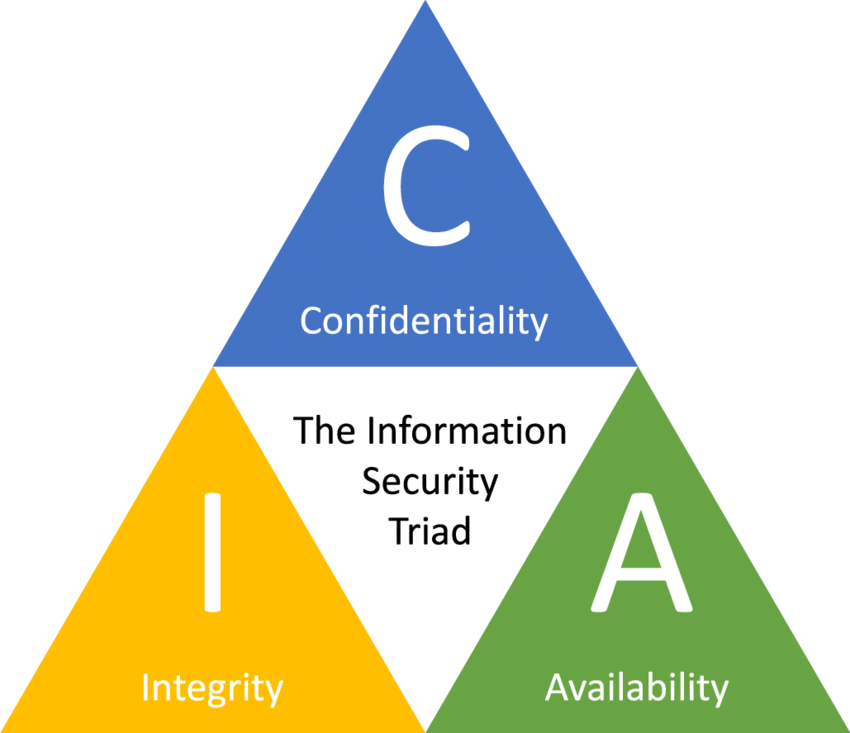
\includegraphics[width=\linewidth]{figures/CIA.png}
   \end{wrapfigure}

   \textbf{Confidentiality:}\\
   Ensures that sensitive information is \rgbO{accessible only to authorized users}. This prevents unauthorized disclosure of data.\\
   \textbf{\textit{Techniques includes}:} Encryption, access control, authentication.
   
   \vspace{1em}
   \textbf{Integrity:}\\
   Ensures that data is \rgbO{accurate and unaltered} during storage, transmission, and processing. This prevents unauthorized modification of data.\\
   \textbf{\textit{Techniques includes}:} Checksums, hash functions, digital signatures.
   
   \vspace{1em}
   \textbf{Availability:}\\
   Ensures that information and resources are \rgbO{accessible and usable when needed} by authorized users. This prevents disruptions in service.
\end{minipage}

\textbf{\textit{Techniques includes}:} data redundancy, protection from DDoS attack, load balancing, implementing firewalls and regular backups.
   
\section{Cyber Attacks}

\subsection{Web Based Attacks}
\textbf{\textit{Mnemonic:}} 

In Dhaka, Smart People Buy Delicious Dumpling Using Fresh Money

\begin{tabularx}{\textwidth}{llX}
Injection attacks &:& Attacker injects malicious code into a web application and fetch required information. \\
DNS Spoofing &:& Attacker changes the DNS address of a website to redirect the user to a fake website. \\
Session Hijacking &:& By stealing the cookies, an attacker can have
access to all of the user data. \\
Phishing &:& Steals sensitive information like user credentials and credit card number by pretending to be trustworthy sources. \\
Brute Force &:& A hacking method that uses trial-and-error to crack passwords, credentials, or encryption keys. \\
Denial of Service (DOS) &:& Attacker overloads a target server or network with traffic from multiple sources, making it unavailable to legitimate users. \\
Volume-based attacks &:& Its goal is to saturate the bandwidth of the attacked site, and is measured in bit per second. \\
Protocol attacks &:& It consumes actual server resources, and is measured in a packet.\\
Application layer attacks &:& Its goal is to crash the web server and is measured in request per second.\\
Dictionary attack &:& Attacker uses a list of commonly used passwords to guess original one.\\
URL Interpretation &:& Attacker changes certain parts of a URL, leading to unauthorized access or data exposure.\\
File Inclusion Attack &:& Attacker uses the include feature to access sensitive files or run malicious code on the web server.\\
MITM &:& Attacker to intercepts connection between client and server and acts as a bridge between them.
\end{tabularx}

\pagebreak
\section{Credit Card Fraud}
\begin{wrapfigure}{r}{0.4\textwidth}
   \centering
   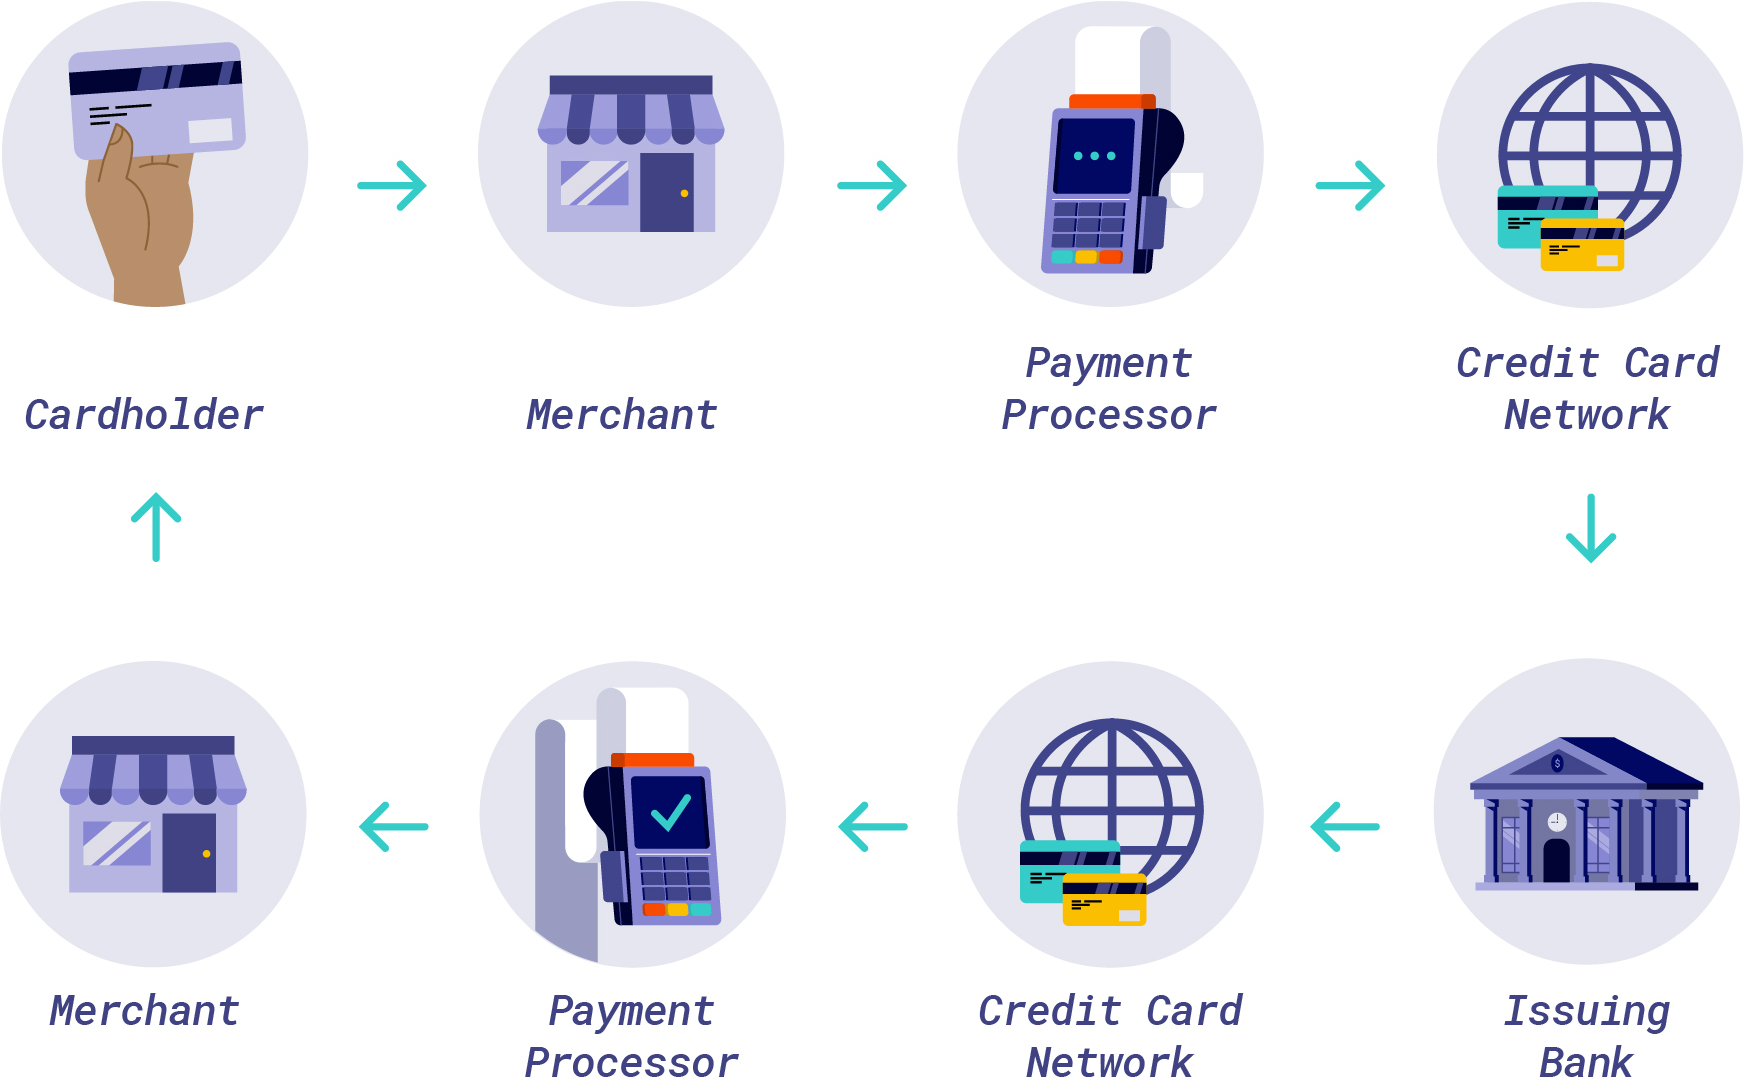
\includegraphics[width=\linewidth]{figures/CreditCard.png}
\end{wrapfigure}

With the rise of mobile computing, including M-Commerce and M-Banking, cyber crimes such as credit card fraud are becoming more frequent. The affordability and accessibility of powerful mobile devices make it easier for both consumers and criminals to engage in these systems.

Wireless technology has enabled anytime, anywhere computing, especially for white-collar professionals. This includes wireless credit card processing, which allows businesses to accept payments on the go. While highly convenient and efficient for mobile businesses, it also increases the risk of security breaches, making cybersecurity in mobile environments more critical than ever.


\section{Cryptography}
Cryptography is the practice of securing information using codes and algorithms so that only intended recipients can understand it. It relies on mathematical techniques for key generation, encryption, digital signing, and verification to ensure data confidentiality, integrity, and authenticity. The term comes from “crypt” (hidden) and “graphy” (writing).

\subsection{Symmetric Key Cryptography}
\begin{wrapfigure}{r}{0.4\textwidth}
   \vspace{-2em}
   \centering
   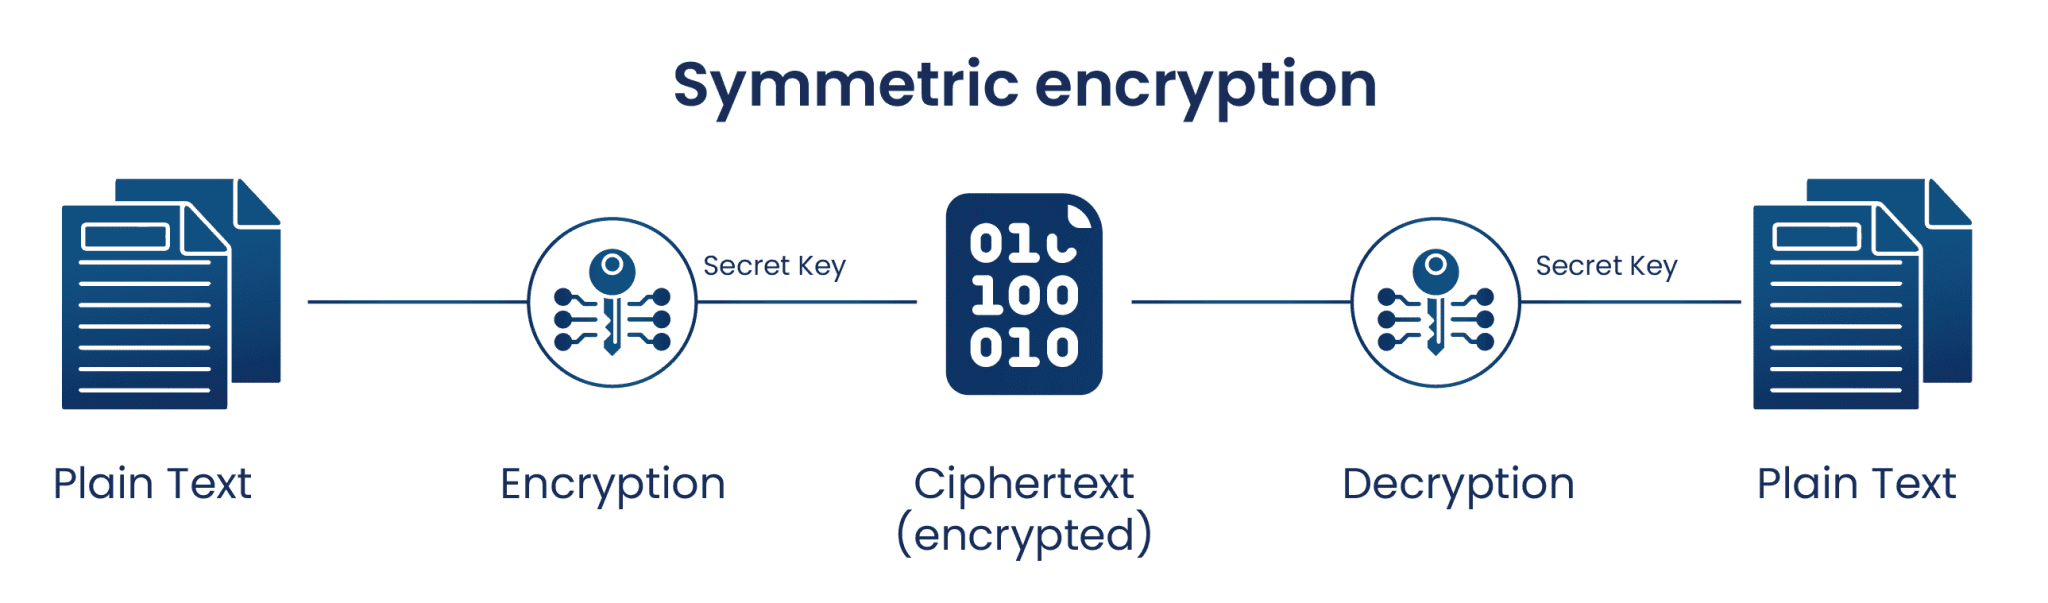
\includegraphics[width=\linewidth]{figures/Symmetric Crypto.png}
\end{wrapfigure}
Symmetric key cryptography uses a \rgbO{single shared key for both encryption and decryption}. It's fast and efficient, but requires a secure method to share the key between sender and receiver. Common examples include Data Encryption Systems (DES) and Advanced Encryption Systems (AES).
   
\subsection{Asymmetric Key Cryptography}
\begin{wrapfigure}{r}{0.4\textwidth}
   \vspace{-2em}
   \centering
   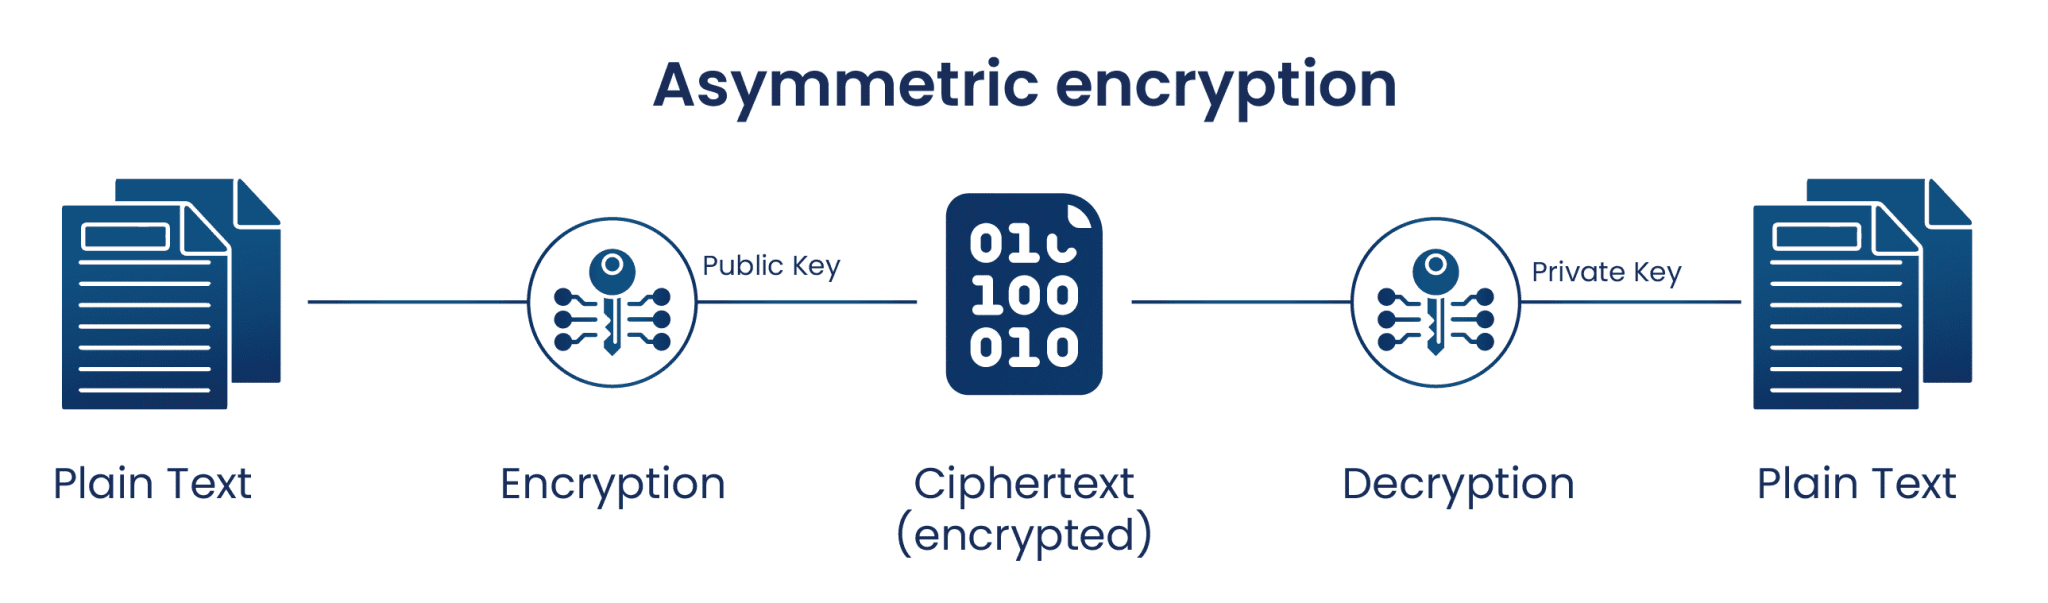
\includegraphics[width=\linewidth]{figures/Asymmetric Crypto.png}
\end{wrapfigure}
Asymmetric key cryptography uses a \rgbO{pair of keys—a public key for encryption and a private key for decryption}. While the public key is openly shared, only the intended receiver can decrypt the message using their private key. A widely used example is the RSA algorithm.

{\subsection{Hash Functions}
There is \rgbO{no usage of any key} in this algorithm. \rgbO{Uses a calculated hash value as per the plain text} which makes it impossible for the contents of plain text to be recovered. Many operating systems use hash functions to encrypt passwords.}

\section{Types of Cryptographic Algorithms}

\textbf{AES (Advanced Encryption Standard):}
A symmetric key block cipher that encrypts data in 128-bit blocks using 128, 192, or 256-bit keys. It's fast, secure, and the modern standard replacing DES.

\textbf{DES (Data Encryption Standard):}
An older symmetric algorithm that encrypts 64-bit blocks using a 56-bit key. It's now considered insecure due to its short key length.

\textbf{RSA (Rivest-Shamir-Adleman):}
A widely used asymmetric algorithm that uses a public key for encryption and a private key for decryption. Based on the difficulty of factoring large integers.

\textbf{SHA (Secure Hash Algorithm):}
A family of cryptographic hash functions (e.g., SHA-2, SHA-3) used to generate fixed-size hash values from input data to ensure data integrity and authenticity. Even small input changes yield drastically different hashes.

% cryptography,
% Cipher text,
% ,
% and other security protocols like SSL and TLS.
